\section{模型效率与架构}
\label{sec:eff}

前几节都把模型当作给定的，只改系统。这一节反过来，讨论通过「改模型」来改变系统代价的方法：参数高效微调、剪枝与蒸馏、混合专家（MoE）、
attention-free 架构，以及决定「训多大的模型、用多少数据」的 scaling law。面试中这部分考的不是算法细节，而是每种方法把式~\eqref{eq:three} 的哪一项换成了哪一项。

\subsection{参数高效微调：LoRA 与 QLoRA}

全量微调一个大模型，显存主要花在梯度和优化器状态上。LoRA~\cite{hu2022lora} 的做法是冻结预训练权重 $W\in\mathbb{R}^{d\times k}$，只训练一个低秩的增量：
\begin{equation}
W' = W + \frac{\alpha}{r}BA,\quad A\in\mathbb{R}^{r\times k},\ B\in\mathbb{R}^{d\times r},\ B_0=0,
\end{equation}
可训练参数只有 $r(d+k)$ 个；推理时可以把 $BA$ 合并回 $W$，不增加时延。$d=k=4096$、$r=16$ 时，可训练参数是 131K，只占全量 16.8M 的 0.78\%。
QLoRA~\cite{dettmers2023qlora} 再把冻结的基座量化成 4 位 NormalFloat（NF4），加上双重量化和分页优化器，使 65B 模型能在单张 48~GB 的 GPU 上微调。

\lab{15-849 编译与压缩}验证了 LoRA 的两个恒等式：初始化时输出与基座的最大差为 0，合并后的最大差是 $3.3\times10^{-15}$。它还验证了低秩逼近的下界：
$d=256$、真实 $\Delta W$ 的秩为 8 时，$r=4$ 的误差 0.434 已经接近 Eckart--Young 下界 0.424，$r=8$ 时降到 0.044。
按 Llama-3-8B 的形状算，$r=8$ 只挂在 q、v 上是 3.41M 参数（0.042\%），$r=16$ 挂在全部线性层上是 41.9M（0.52\%）。

\begin{qa}{LoRA 省的是什么显存？不省什么？}
\ans 省的是梯度和优化器状态。只有 $r(d+k)$ 个参数需要 FP32 主权重和 Adam 的 $m,v$，7B 模型的优化器状态可以从 84~GB 降到 0.1~GB 的量级。
不省的是基座权重和激活：BF16 的基座仍要 $2N$（QLoRA 用 4 位把它降到约 $0.5N$），反向传播也仍要流经全部层。
\wrong 「LoRA 省了前向显存」，或者「LoRA 让训练快很多」。它的前反向计算量和全量微调相近。
\end{qa}

\subsection{剪枝、稀疏与蒸馏}

剪枝想直接减少参数，难点在于稀疏能不能在硬件上兑现成加速。Deep Compression~\cite{han2016deep} 用剪枝、量化（权重共享）和 Huffman 编码，把 CNN 压缩了一到两个数量级；
但非结构化的稀疏在 GPU 上很难变成实际加速。NVIDIA 的 2:4 结构化稀疏（每 4 个元素保留 2 个）由 Ampere 之后的稀疏 tensor core 直接支持，理论算力翻倍~\cite{mishra2021accelerating}。
SparseGPT~\cite{frantar2023sparsegpt} 把 GPTQ 式的二阶补偿用到了一次性剪枝上。知识蒸馏~\cite{hinton2015distilling} 则用大模型的软标签训练小模型，是部署侧最常用的「改模型」手段之一。

结构约束是有代价的。\lab{15-849 编译与压缩}中，对一个 $1024^2$ 的重尾矩阵剪掉 50\%，非结构化剪枝的输出误差是 20.4\%，2:4 是 29.0\%，4:8 是 25.1\%。
在一个小 MLP 上，2:4 稀疏不微调时准确率是 62.9\%，微调 3 轮后回到 67.2\%（稠密模型是 66.2\%）。这说明结构约束越强，就越依赖恢复训练。

\begin{qa}{2:4 稀疏和非结构化稀疏怎么选？}
\ans 在精度和能否加速之间取舍。非结构化稀疏在同样稀疏度下精度更好，但访存不规则、索引开销大，GPU 很难加速。2:4 有硬件支持（稀疏 tensor core，每 4 个元素用 2 位元数据），
能兑现约 2 倍的算力上限，但约束更强、精度损失更大，通常要微调来恢复。实际加速还要看 GEMM 是否受算力限制：decode 受带宽限制时，2:4 省下的是权重字节，而不是 FLOPs。
\wrong 「剪掉 50\% 就快 2 倍」。非结构化的 50\% 在 GPU 上几乎不会变快。
\end{qa}

\subsection{混合专家（MoE）与专家并行}

能不能让参数变多，而每个 token 的计算不变？这就是 MoE 的想法。Sparsely-gated MoE~\cite{shazeer2017outrageously} 用一个门控网络为每个 token 选出 top-$k$ 个专家（每个专家是一个 FFN），
于是参数量随专家数 $E$ 线性增长，每 token 的 FLOPs 却只随 $k$ 增长。GShard~\cite{lepikhin2021gshard} 用 top-2 门控和自动分片把 MoE 扩展到了 600B 参数；
Switch Transformer~\cite{fedus2022switch} 进一步简化为 top-1，并引入了容量因子和辅助负载均衡损失。容量因子规定每个专家最多接收 $\text{capacity}=\text{factor}\times\text{tokens}/E$ 个 token，
溢出的 token 被丢弃或走残差连接。

专家并行（EP）把专家分到不同的卡上，每层前向需要两次 all-to-all，一次把 token 分发给专家（dispatch），一次把结果收回来（combine），反向还要再两次。
DeepSpeed-MoE~\cite{rajbhandari2022deepspeed} 从推理系统的角度优化 MoE；MegaBlocks~\cite{gale2023megablocks} 用块稀疏 kernel，避免了容量因子带来的丢 token 和 padding。
DeepSeek-V2/V3~\cite{deepseekai2024v2,deepseekai2024v3} 采用了细粒度专家加共享专家的结构。

\begin{est}{MoE 的 all-to-all 每次要传多少？}
每张卡 8192 个 token、$d=4096$、top-2、BF16、EP=8：每张卡每次发送 $\approx8192\times2\times4096\times2\times\frac{7}{8}\approx117$~MB。
每层前向 2 次、反向 2 次；如果跨 IB（50~GB/s），每次约 2.3~ms，32 层每步约 0.3~s，和 TP 的通信是同一个量级。所以 EP 通常放在节点内，或者和 DP 交织，以利用节点内的带宽。
\end{est}

\begin{qa}{MoE 为什么「参数多但不贵」？它贵在哪？}
\ans 不贵的是 FLOPs：每个 token 只经过 top-$k$ 个专家，计算量随 $k$ 增长，而不是随 $E$。贵的地方有三处。一是显存，全部专家都要放下，部署时要按总参数而不是激活参数来配卡。
二是通信，EP 每层前反向共 4 次 all-to-all，对网络拓扑很敏感。三是负载不均，热门专家所在的卡会拖慢整步，需要负载均衡损失、容量因子，或者无丢弃的块稀疏实现。
推理时还有一点：decode 读的是被激活专家的权重，batch 一大，几乎所有专家都会被激活，访存上的优势也就随之减少。
\wrong 「MoE 省算力，所以训练和部署都便宜」。
\end{qa}

\subsection{Attention-free 与状态空间模型}

第~\ref{sec:infer} 节看到，长上下文下 KV cache 是 decode 的主要负担。Transformer~\cite{vaswani2017attention} 的 attention 让 KV cache 随长度线性增长，
而循环形式的模型每一步的状态大小是固定的，这正是 attention-free 架构吸引人的地方。线性 attention~\cite{katharopoulos2020transformers} 把 $\mathrm{softmax}(QK^\top)V$
换成 $\phi(Q)(\phi(K)^\top V)$，复杂度降到 $O(Td^2)$。S4~\cite{gu2022efficiently} 用结构化状态空间模型，训练时写成长卷积的形式来并行。
Hyena~\cite{poli2023hyena} 用隐式参数化的长卷积加门控来替代 attention。Mamba~\cite{gu2023mamba} 引入了随输入变化的选择性状态空间，用硬件感知的并行扫描来训练；
推理时每个 token 的代价是 $O(1)$，没有 KV cache。

\lab{CS229S P1}有两个与此相关的测量。第一个是 depthwise 因果卷积的三种写法（$C=16$，float64）。FFT 的耗时只取决于 $N$，$N=16384$ 时约 14--15~ms；
$O(NK)$ 的直接写法随 $K$ 线性增长，其中移位相加在 $K\approx16$ 处、滑窗在 $K\approx64$ 处与 FFT 交叉。所以短卷积（Mamba/H3 的 $K=4$）直接写快 5.2--8.5 倍，
而长卷积（Hyena 的 $K=N$）在所有 $N$ 上都是 FFT 更快。
第二个是 associative recall。一个手工设定权重、没有经过训练的两层 attention-only 模型（一个「上一 token」头加一个匹配头，也就是 induction head）
就能精确地解这个任务：$\beta\ge8$ 时，32 个键值对的准确率是 1.0；$\beta=1$ 时只有 0.227。这说明 attention 天然擅长精确检索；
而状态大小固定的 SSM 必须把历史压缩进状态里，这正是它在 recall 类任务上的弱点。

\begin{qa}{Mamba/SSM 相对 Transformer 的推理优势是什么？代价呢？}
\ans 优势是状态大小固定。写成递归形式时，decode 不需要随长度增长的 KV cache，每个 token 的代价是 $O(1)$，长序列、大 batch 下吞吐和显存都更好；训练时则用并行扫描或卷积形式来并行。
代价是固定大小的状态是对历史的有损压缩，精确检索（长距离复制、associative recall）不如 attention。所以出现了把 attention 和 SSM 混合起来的架构。
\wrong 「SSM 在所有任务上都比 attention 好」，或者「SSM 训练时也是每 token $O(1)$，没法并行」。
\end{qa}

\subsection{Scaling law 与计算最优}

最后一个问题是：给定一笔算力，应该训多大的模型、用多少数据？Kaplan 等人~\cite{kaplan2020scaling} 发现，损失随参数量 $N$、数据量 $D$ 和算力 $C$ 呈幂律下降。
Chinchilla~\cite{hoffmann2022training} 在固定算力下重新做了拟合，结论是参数和数据应该大致同比例增长，约为每个参数 20 个 token：
\begin{equation}
C\approx6ND,\quad D^\ast\approx20N^\ast\ \Rightarrow\ N^\ast\approx\sqrt{C/120}.
\end{equation}
要注意，这是\emph{训练}算力最优，而不是推理成本最优。要大规模部署的模型常常远超 20 token/参数：Llama-3-8B 训了 15T token，约 1868 token/参数~\cite{dubey2024llama3}，
相当于用更多的训练算力换一个更小、推理更便宜的模型。图~\ref{fig:chinchilla} 左把若干公开模型放在 Chinchilla 曲线旁边：GPT-3 175B 只训了 300B token（约 2 token/参数），明显「欠训」；
Chinchilla 70B 落在曲线上；Llama 系列则大幅「过训」。

\begin{figure*}[!t]
\centering
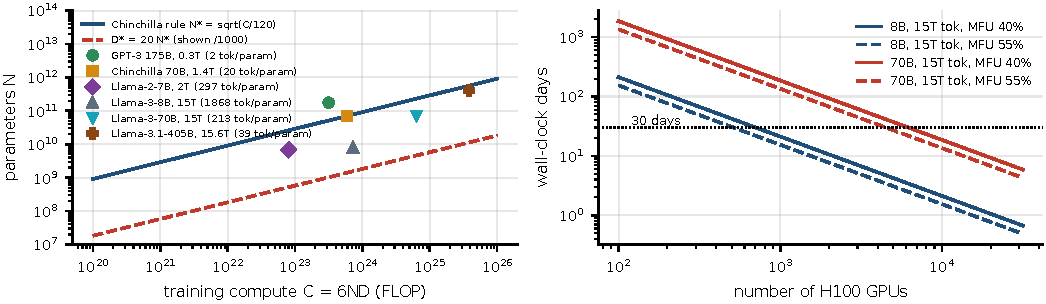
\includegraphics[width=\textwidth]{fig_chinchilla}
\caption{左：Chinchilla 计算最优规则 $N^\ast=\sqrt{C/120}$（实线）与 $D^\ast=20N^\ast$（虚线，缩小 1000 倍显示），以及公开模型的 $(C,N)$ 和 token/参数比；离曲线越远，说明这个模型的训练越偏离「训练算力最优」。
右：在 H100 上用 15T token 训练 8B 和 70B 模型所需的墙钟天数随 GPU 数的变化（MFU 取 40\% 和 55\%）。70B 用 8192 卡、MFU 40\% 时约需 23 天。}
\label{fig:chinchilla}
\end{figure*}

\begin{est}{给定 $6\times10^{23}$ FLOP，计算最优的模型多大？}
$N^\ast=\sqrt{6\times10^{23}/120}\approx7.1\times10^{10}$，也就是约 70B；$D^\ast=20N^\ast\approx1.4$T token。这和 Chinchilla 70B/1.4T 一致（$6\times70\times10^9\times1.4\times10^{12}\approx5.9\times10^{23}$）。
如果改训 8B 模型，同样的算力可以训约 12T token，推理成本约为 70B 的 1/9。用 1 万张 H100、MFU 40\%，$6\times10^{23}$ FLOP 约需 $1.5\times10^5$~s，不到 2 天。
\end{est}

\begin{qa}{Chinchilla 的结论是什么？「每个模型都该训 20 token/参数」对吗？}
\ans 不对，因为 Chinchilla 只考虑了训练算力。它的结论是：固定训练算力时，参数和数据应同比例扩展，最优约为 20 token/参数，$C\approx6ND$。
但如果模型要服务大量请求，总成本是训练加推理，而推理成本随模型大小线性增长，所以应该训练更小的模型、喂更多的 token（Llama-3-8B 约 1868 token/参数）。
可用的高质量数据有限，也是一个现实约束。
\wrong 「Chinchilla 说模型训 20 token/参数最好」。这忽略了推理成本和数据约束。
\end{qa}

\begin{keypts}
\begin{itemize}
\item LoRA 的参数量是 $r(d+k)$，省梯度和优化器状态，不省基座权重和激活；QLoRA 再把基座压到 4 位。
\item 2:4 稀疏有硬件支持（约 2 倍的算力上限）；非结构化稀疏难以兑现加速。
\item MoE：FLOPs 随 $k$ 增长，显存随 $E$ 增长；EP 每层前反向共 4 次 all-to-all（8192 token、$d=4096$、top-2、EP=8 时约 117~MB/次）。
\item SSM：decode 每 token $O(1)$，没有 KV，但精确检索弱；短卷积直接算，长卷积用 FFT。
\item Chinchilla：$N^\ast=\sqrt{C/120}$、$D^\ast=20N^\ast$；要部署的模型常常故意过训。
\end{itemize}
\end{keypts}

\begin{research}
\begin{itemize}
\item 推理感知的 scaling law：把部署时的 token 总量 $D_{\text{inf}}$ 纳入目标函数 $\min_{N,D}6ND+2ND_{\text{inf}}$（在损失约束下），最优的 token/参数比怎样随 $D_{\text{inf}}$ 变化？
这是一个可以用公开拟合系数来做的解析练习。
\item MoE 的通信与计算之比随专家粒度变化：细粒度专家增加了 all-to-all 的消息数（$\alpha$ 项），但改善了负载均衡。可以在本文的 $\alpha$--$\beta$ 模拟器上扫描专家数和 top-$k$，
找出 all-to-all 从带宽主导转为延迟主导的拐点。
\end{itemize}
\end{research}
